\chapter{Planung}
\section{Organisation}
\subsection{Kommunikation}
\subsection{Rollenverteilung}
\subsection{Tools und Technologien}
\section{Spezifikation}
\subsection{Anforderungsanalyse}
Die Anforderungen für das Projekt haben wir nach dem Kick-Off Meeting mit dem Professor in einem Kollektiven Brainstorming gesammelt. Da bei diesem Projekt kein klassischer Kunde vorhanden ist, der die grundlegenden Anforderungen vorgibt, waren die Anforderungen recht flexibel und wir haben uns an einigen Referenzprodukten und deren Funktionsumfang orientiert.
\subsection{Anforderungsdetails}
\textbf{Bewegungserkennun}\newline
Ein Videostream soll programmatisch auf Bewegungen überprüft werden. Die Überprüfung soll kleine Änderungen wie durch Wind bewegte Blätter und Kamerarauschen ignorieren und größere Bewegungen erkennen.
\newline
\textbf{Log}\newline
Erkannte Bewegungen sollen in einem Log festgehalten und archiviert werden.
Dabei soll der Zeitpunkt der Aufnahme, die Aufnahme selbst und ein dazugehörendes Thumbnail gespeichert werden. Der Log Wird automatisch erzeugt und kann durch manuelles löschen von Einträgen manipuliert werden.
\newline
\textbf{Aufnahmefunktion}\newline
Wenn eine Bewegung erkannt wurde soll das System in der Lage sein den Videostream in einer persistenten Datei zu speichern.
Die gespeicherten Aufnahmen müssen jederzeit abrufbar sein.
In der Aufnahme sollen erkannte Bewegungen visuell hervorgehoben werden.
\newline
\textbf{E-Mailbenachrichtigungen}\newline
Bei Einer erkannten Bewegung soll Das System in der Lage sein Automatisiert Eine E-Mailbenachrichtigung zu versenden.
\newline
\textbf{lokales Verfahren}\newline
Die aufgezeichneten Daten sollen das lokale Netzwerk nicht verlassen.
Alle Verfahrensschritte benutzen ausschließlich lokal ausgeführte Software.
\newline
\textbf{Videofeed}\newline
Der live Videostream soll direkt angezeigt werden können.
\newline
\textbf{Backup}\newline
Es soll die Möglichkeit die im Log gesammelten Daten als Datei zu exportieren.
\newline
\textbf{Einstellungsmöglichkeiten}\newline
In der Weboberfläche sollen einige Benutzer spezifische Einstellungen für das Programm getroffen werden können.
Diese umfassen: 
\begin{itemize}
\item Einstellen der Empfindlichkeit der Bewegungserkennung
\item Bildkorrektureigenschaften wie Kontrast und Helligkeit
\item Einstellen der Streamquelle
\item Limit für die maximale Länge einer zusammenhängenden Aufnahme bei konstanter Bewegung
\item Limits für das Backup (maximale Anzahl Dateien / Dateigröße)
\item Login Daten ändern
\item festlegen der E-Mailbenachrichtigungs Empfänger.
\item Ein-/ausschalten des Logs
\item Ein-/ausschalten der E-Mailbenachrichtigungen
\end{itemize}
\textbf{Weboberfläche}\newline
Es soll eine Weboberfläche als Benutzerschnittelle geschaffen werden die alle Funktionen des Systems einem Anwender exponiert.
Die Funktionen der Weboberfläche sind wie Folgt definiert:
\begin{itemize}
\item Der zugriff soll durch einen login mit Benutzernamen und Passwort geschützte geschützt werden werden.
\item Der Livefeed der Kamera soll prominent auf der dargestellt werden.
\item Der Log soll mit allen oben definierten Eigenschaften präsentiert werden.
\item Aufnahmen sollen angesehen werden können
\item Alle oben definierten Einstellungen sollen über die Weboberfläche manipuliert werden können.
\item Möglichkeit ein Backup zu erstellen und herunterzuladen.
\end{itemize}
Es gab noch weitere Anforderungen die, wie sich später herausstellte, nicht realisierbar waren. Eine Gesichtserkennung, die wegen der geringen Qualität und Größe der Gesichter in der Aufnahme technisch nicht umsetzbar war.  Zuletzt eine Portierung auf einen Raspberry Pi, die wegen des hohen Leistungsanspruches der Software nicht umsetzbar war. Die Portierung des Produktivsystems erfolgt stattdessen auf einen lokalen Server.
 
\subsection{User Stories}
Als Benutzer möchte ich mich mit einem Benutzernamen und Password in die Weboberfläche einloggen, um sicherzustellen, dass nur autorisierte Benutzer Zugriff auf die Weboberfläche haben.
\newline
Als Benutzer möchte ich, dass ich Einstellung für die Software über die Weboberfläche ändern kann um das Softwareverhalten dynamisch zu beeinflussen.
\newline
Als Benutzer möchte ich meine Emailadresse zum Verteiler für Benachrichtigungen hinzufügen und wieder entfernen können, um so einfach wie möglich auf erkannte Bewegungen aufmerksam gemacht zu werden.
\newline
Als Benutzer möchte ich, Aufnahmen über die Weboberfläche einsehen können, um zu entscheiden, ob die erkannte Bewegung von einem unbefugten Zutritt herrührt.
\newline
Als Benutzer möchte ich den Überwachungs-Videostream über eine Weboberfläche einsehen können, um das Blickfeld der Kamera zu sehen.
\newline
Als Benutzer möchte ich, eine Übersicht über alle erfassten Ereignisse der Kamera mit Zeitstempel einsehen, um nach einem Event in einem gewissen Zeitraum zu suchen.
\newline
Als Benutzer möchte ich, dass meine Daten nicht auf den Servern von Drittanbietern gespeichert werden, um meine Privatsphäre zu schützen.
\newline
Als Benutzer möchte ich, die gesammelten Aufnahmedaten exportieren, um sie anderweitig zu verwenden.


\subsection{Meilensteine}
Die Termine der Meilensteine wurden an den Zweiwöchentlichen Meetings mit den Betreuern ausgerichtet. Einzige Ausnahme War Die Implementierungsphase, die Für die Basisimplementierung vier Wochen beansprucht hat. Somit ergeben sich Meilensteine für die, unter anderem im klassischen Wasserfallmodell, vorgegebenen Phasen Spezifikation, Entwurf, Implementierung und Test. Ein letzter, zusätzlicher Meilenstein für die abschließende Präsentation. Die Implementierungsphase war jedoch in  4 feingranulare Meilensteine aufgeteilt. Es wurden jeweils zwei Meilensteine für die Basisfunktionalität von Front- und Backend, und der jeweiligen Featureimplementierung aufgestellt. Diese sind auf die einzigen Meilensteine die parallelisiert bearbeitet werden konnten, da das Front- und Backend weitestgehend unabhängig bearbeitet werden können.
\newline
[Bild]
\newline
Die Meilensteine konnten im Projektverlauf ausnahmslos eingehalten werden und er gab keine Verschiebungen.

\section{Entwurf}
\subsection{Systemarchitektur}
Bei dem ersten Treffen mit dem 'Kunden' wurde von uns eine Software zur Überwachung eines Raumes mithilfe einer herkömmlichen IP-Kamera gewünscht.
Da hierfür auch eine Möglichkeit zur Interaktion mit dem System gegeben sein sollte, entschieden wir uns für eine Webseite, mit welcher
der Videofeed sichtbar und Einstellungen vorgenommen werden sollten. Da die Software im Gegensatz zu anderen kommerziellen Produkten im lokalen Netz bleiben sollte,
spielte die Sicherheit keine große Rolle.\\
Die Architektur sollte die Aufteilung der Schichten wie Logik, Datenhaltung sowie die Präsentation durch den Webserver darstellen.
Hierfür wurde zuerst Abbildung \ref{img:architecture-sketch} erstellt.\\\\
\begin{figure}[h]
	\centering
	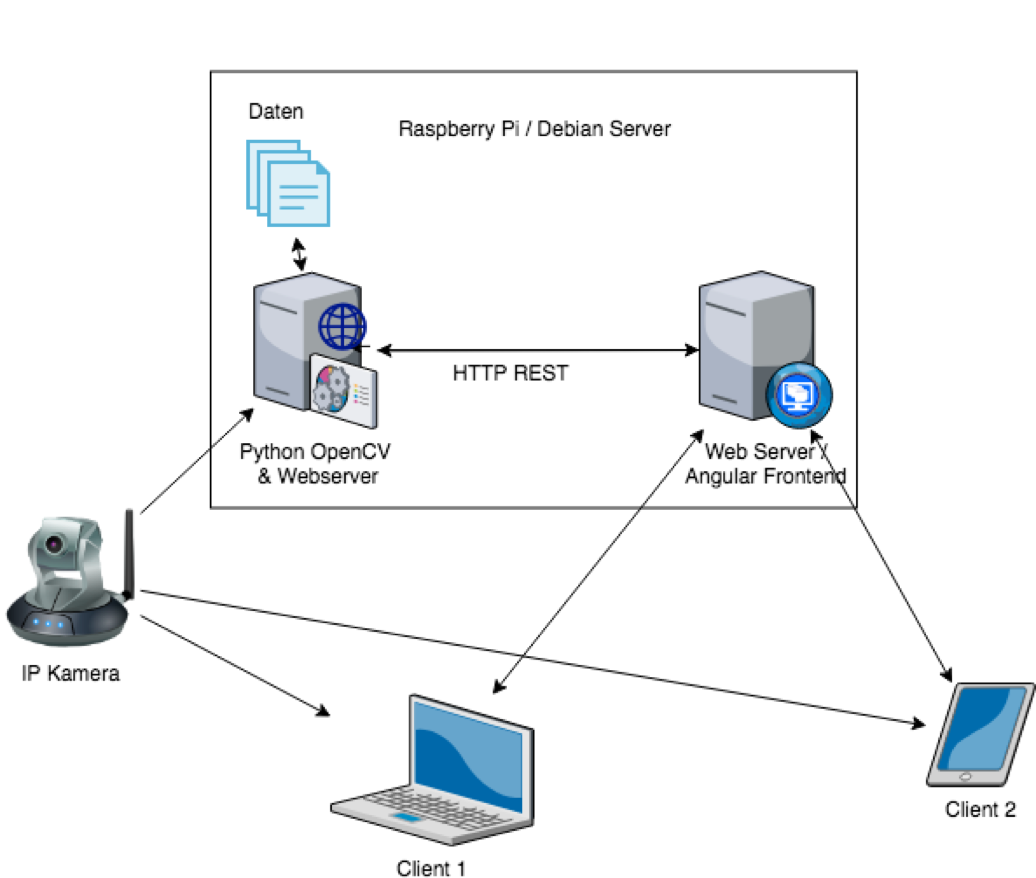
\includegraphics[height=10cm]{content/pictures/architecture-sketch.png}
	\caption{Erste Planung der Architektur}
	\label{img:architecture-sketch}
\end{figure}
Da der Architekt im Gebiet der Webtechnologien kaum Erfahrung hatte, entschieden die verantwortlichen Entwickler sich selbst für Angular und sprachen sich bei
der Entwicklung ab. Lediglich REST wurde für die Kommunikation zwischen Frontend und Backend definiert. 
Um die Aufteilung der Klassen und Kommunikation innerhalb des Backends darzustellen wurde ein grobes Klassendiagramm erstellt (Abbildung \ref{img:backend-classdiagramm}).\\\\
\begin{figure}[]
	\centering
	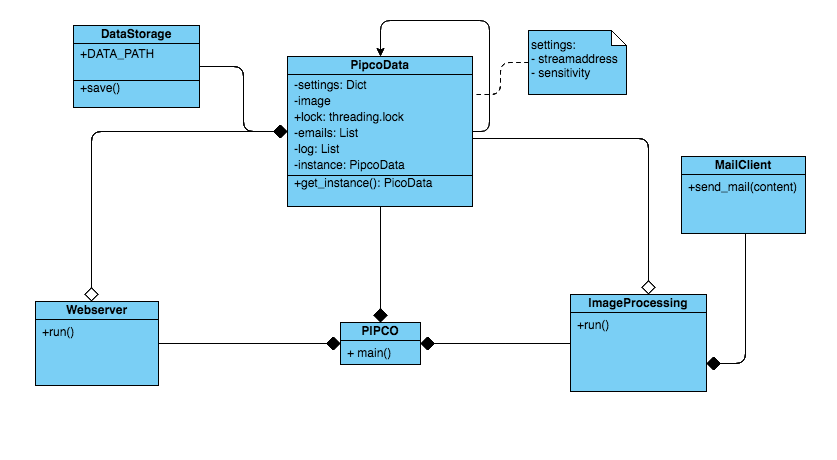
\includegraphics[width=\textwidth]{content/pictures/classdiagramm.png}
	\caption{Klassendiagramm Aufbau des Backends}
	\label{img:backend-classdiagramm}
\end{figure}
Für die Unabhängige Entwicklung der Kommunikation von Frontend und Backend wurde eine Liste mit den notwendigen REST-Nachrichten erstellt (Tabelle \ref{table:kommunikation}).\\\\
\begin{table}[]
	\centering
	\caption{Kommunikation Backend und Frontend}
	\label{table:kommunikation}
	\resizebox{\textwidth}{!}{\begin{tabular}{llll}
		\textbf{Type} & \textbf{address}                                                             & \textbf{keys}                                                                                                                                                                                                                                          & \textbf{returns}           \\
		POST          & /login                                                                       & user, password                                                                                                                                                                                                                                         & OK / Error 403             \\
		GET           & /videostream                                                                 &                                                                                                                                                                                                                                                        & mjpeg stream               \\
		GET           & /logs/\textless{}page\_no\textgreater{}/\textless{}batch\_size\textgreater{} &                                                                                                                                                                                                                                                        & list with logs             \\
		DELETE        & /log/\textless{}log\_id\textgreater{}                                        &                                                                                                                                                                                                                                                        & id / Error 403             \\
		POST          & /mail                                                                        &                                                                                                                                                                                                                                                        & id / Error 403             \\
		GET           & /mails                                                                       &                                                                                                                                                                                                                                                        & list of mail addresses     \\
		DELETE        & /mail/\textless{}mail\_id\textgreater{}                                      &                                                                                                                                                                                                                                                        & id / Error 403             \\
		PUT           & /mail/\textless{}mail\_id\textgreater{}                                      &                                                                                                                                                                                                                                                        & notify status / Error 403  \\
		POST          & /config                                                                      & \multirow{4}{*}{\begin{tabular}[c]{@{}l@{}}sensitivity(float), streamaddress,brightness (float),\\ contrast (float), log\_enabled(bool),\\ global\_notify(bool), cliplength (int in seconds),\\ max\_logs (int),max\_storage (int in MB)\end{tabular}} & changed values / Error 403 \\
		&                                                                              &                                                                                                                                                                                                                                                        &                            \\
		&                                                                              &                                                                                                                                                                                                                                                        &                            \\
		&                                                                              &                                                                                                                                                                                                                                                        &                            \\
		GET           & config                                                                       &                                                                                                                                                                                                                                                        & config                     \\
		GET           & /recording/\textless{}filename\textgreater{}                                 &                                                                                                                                                                                                                                                        & videofile                  \\
		GET           & /backup                                                                      &                                                                                                                                                                                                                                                        & backup.zip                 \\
		&                                                                              &                                                                                                                                                                                                                                                        &                           
	\end{tabular}}
\end{table}
Während der Entwicklung stellte sich heraus, dass der Aufwand für die Implementierung der bidirektionalen Kommunikation zwischen Frontend und Backend zu hoch ist, weshalb wir uns dazu entschieden die Daten direkt vom Backend zu holen und die Logs mithilfe von Polling aktuell zu halten.
Eine weitere Änderung war die Kamera, welche lediglich vom Backend angefragt wird. Der Client sollte sich ausschließlich die Bilder, mit eingezeichneten Bewegungen holen.
Hierdurch änderte sich die Architektur wie in Abbildung \ref{img:architecture-change} zu sehen.\\

Um den Ablauf besser nachvollziehen zu können wurde desweiteren ein Sequenzdiagramm erstellt (Abbildung \ref{img:sequencediagram}).

\begin{figure}[]
	\centering
	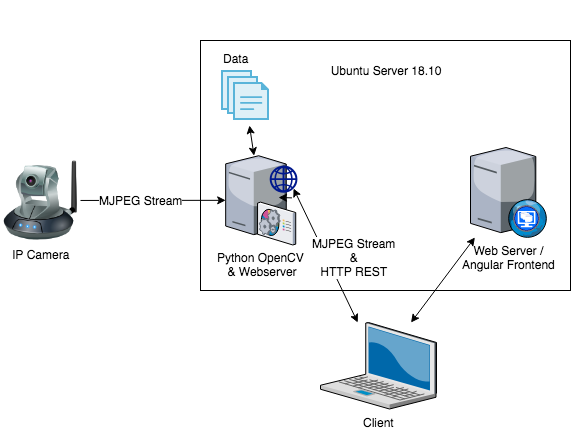
\includegraphics[width=\textwidth]{content/pictures/architecture-change.png}
	\caption{Klassendiagramm: Direkter Zugriff auf das Backend}
	\label{img:architecture-change}
\end{figure}

\begin{figure}[]
	\centering
	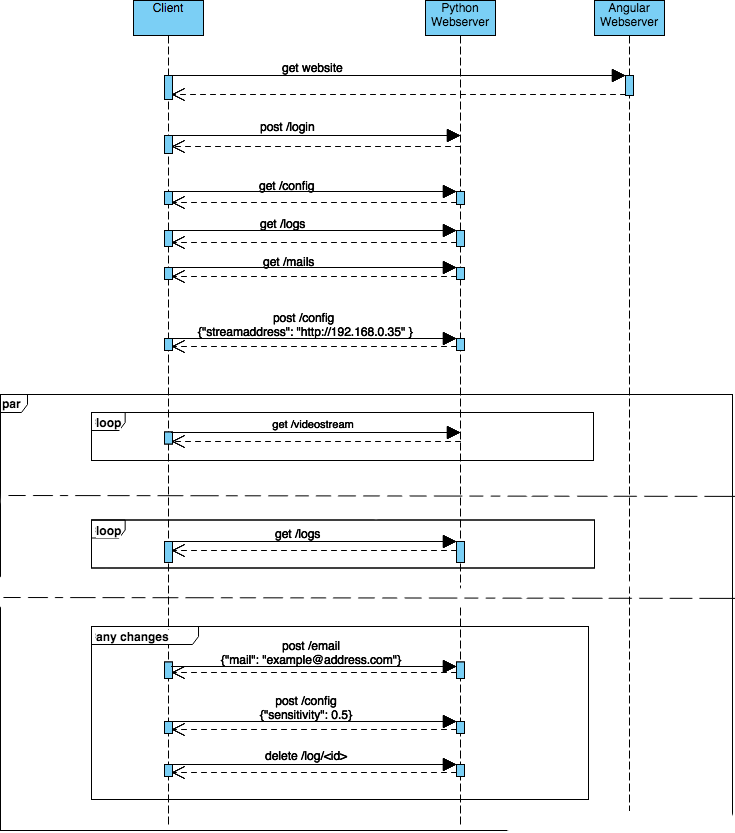
\includegraphics[width=\textwidth]{content/pictures/sequencediagram.png}
	\caption{Ablauf Login und Änderungen}
	\label{img:sequencediagram}
\end{figure}

\subsection{Rest Schnittstelle}